\section{Experiments}
In this section, we will analyze the benefits of 
overclocking on a set of representative convolution neural networks.
Meanwhile, we will also estimate the trade-off of the required strategies 
used to mitigate the overclocking errors.

\subsection{Experiment setup}
We use PipeCNN as the baseline CNN accelerator and have it implemented on KCU1500 FPGA board.
Four representative neural networks including LeNet, AlexNet, VGG-16 and VGG-19 are used to 
benchmark the performance and energy efficiency of the accelerator. The implementation clock
frequency of LeNet and AlexNet is 210 MHz while the clock frequency for VGG-16 and VGG-19 is 190 MHz.
Then we gradually overclock the implementation with 10 MHz step until the accelerator gets 
stuck or crashes frequently. For the 210 MHz implementation, the highest overclocking setup is 
260MHz. For the 190 MHz implementation, the highest overclocking setup is 240 MHz.
Finally, we evaluate the performance and energy efficiency of the accelerators using 
all the available overclocking configurations.

\subsection{Accuracy, performance and energy efficiency}
The prediction accuracy of the benchmark neural networks on the CNN accelerators with overclocking is 
presented in Fig \ref{fig:overclock-accuracy}. It can be found that the prediction accuracy 
regardless of top1 or top5 typically remains the same under moderate overclocking. However, when the clock 
continues to rise, it may reach to a tipping point where the prediction accuracy drops clearly. 
Fortunately, the prediction accuracy can be improved with just on-accelerator retraining.
When the clock further increases, the prediction accuracy drops dramatically. In spite of the retraining, 
the prediction accuracy is still not acceptable in practice. 
\begin{figure}
        \center
	\subfloat[LeNet]{
		\label{fig:lenet_accuracy}
		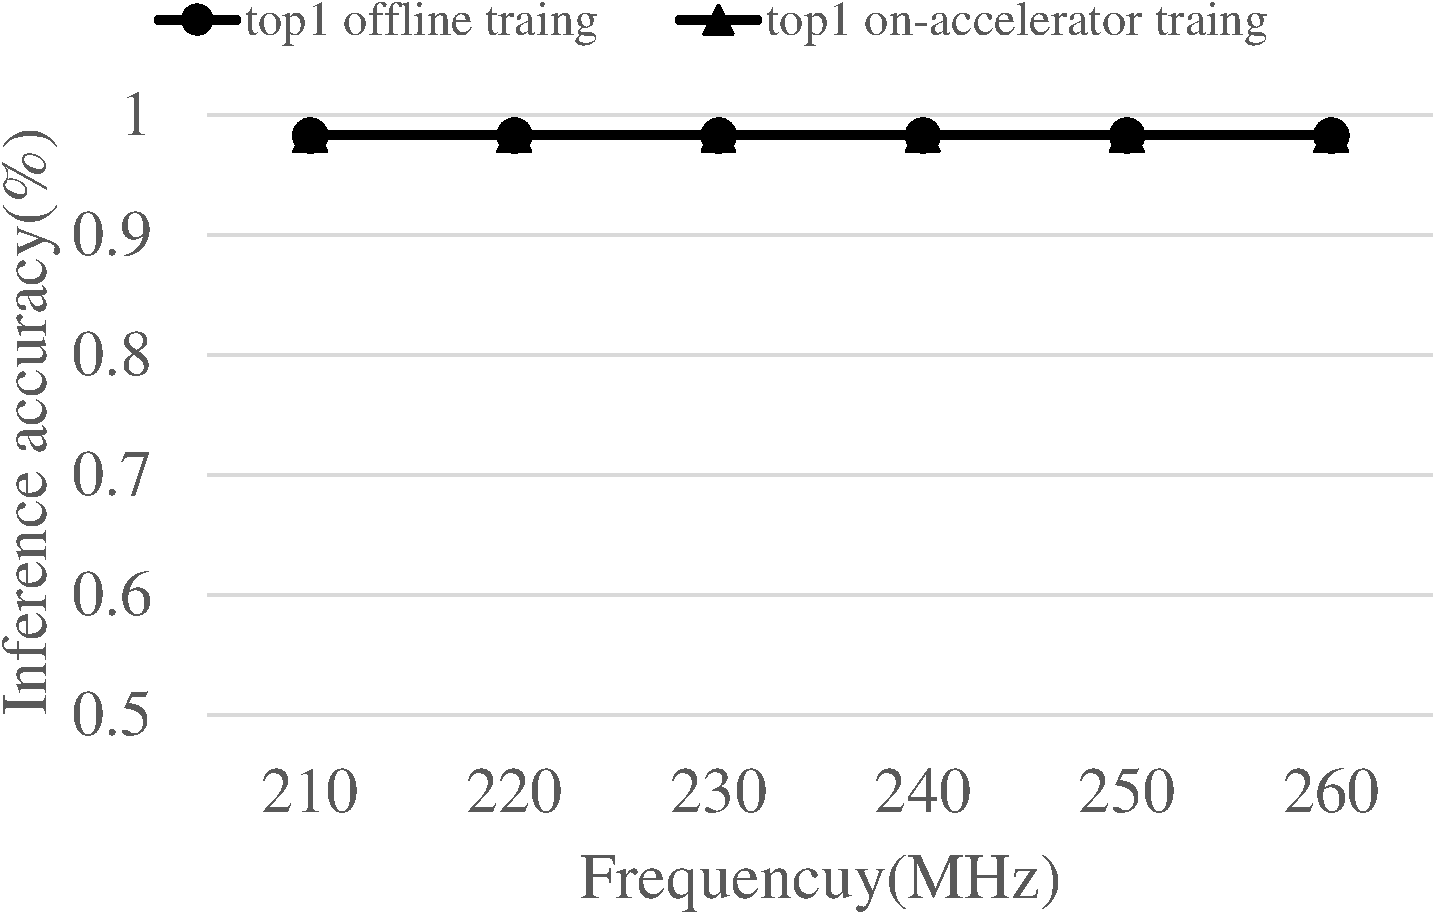
\includegraphics[width=0.6\linewidth]{lenet_accuracy}
	}
	\qquad
	\subfloat[AlexNet]{
                \label{fig:alexnet_accuracy}
                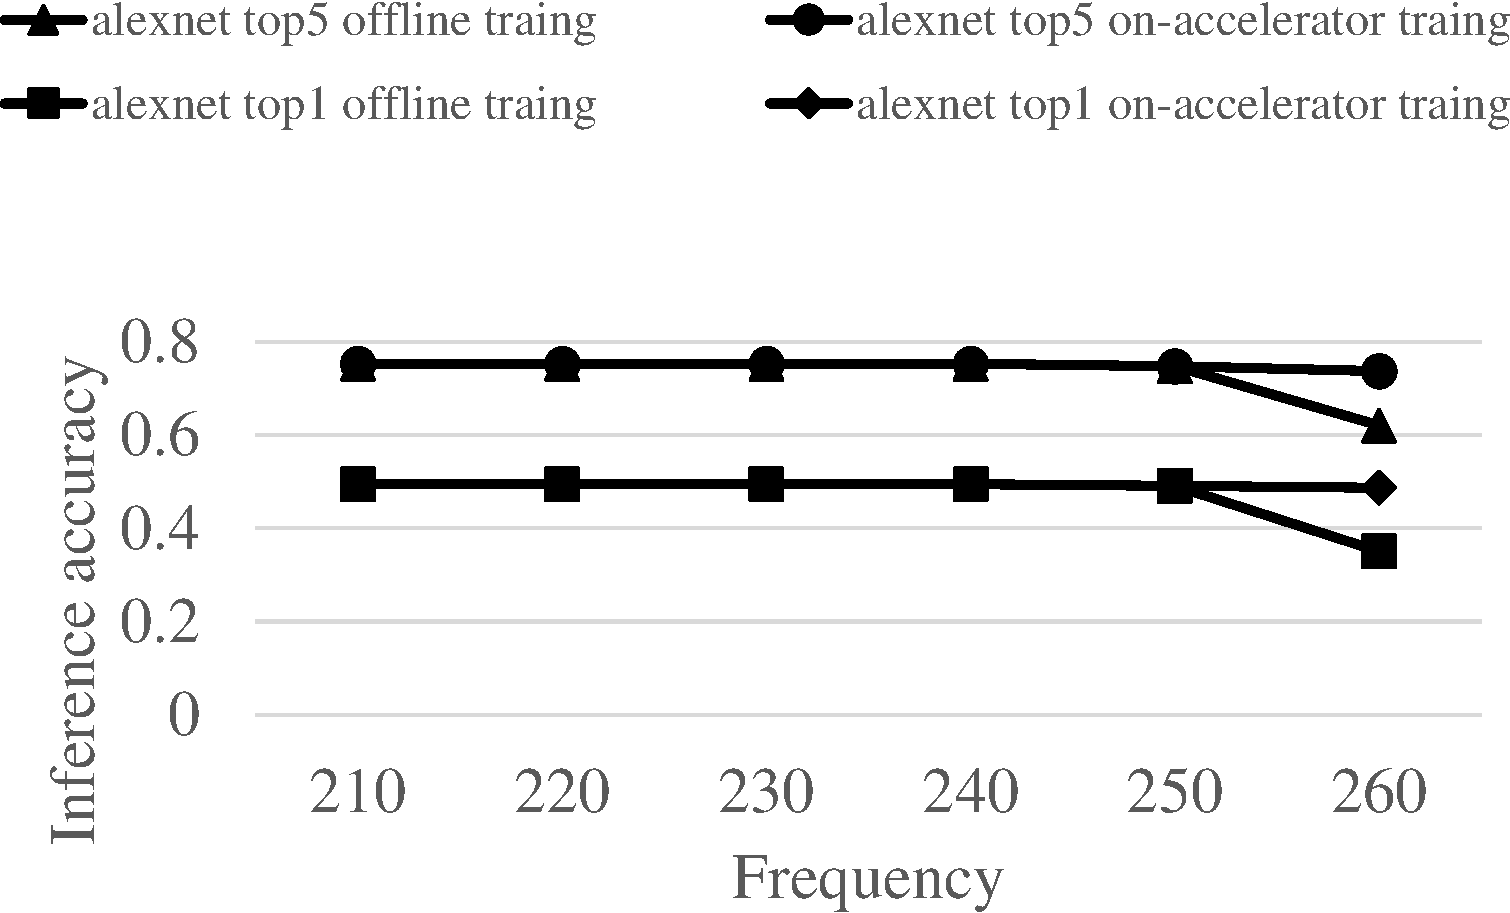
\includegraphics[width=0.6\linewidth]{alexnet_accuracy}
        }
	\qquad
	\subfloat[VGG-16]{
                \label{fig:vgg16_accuracy}
                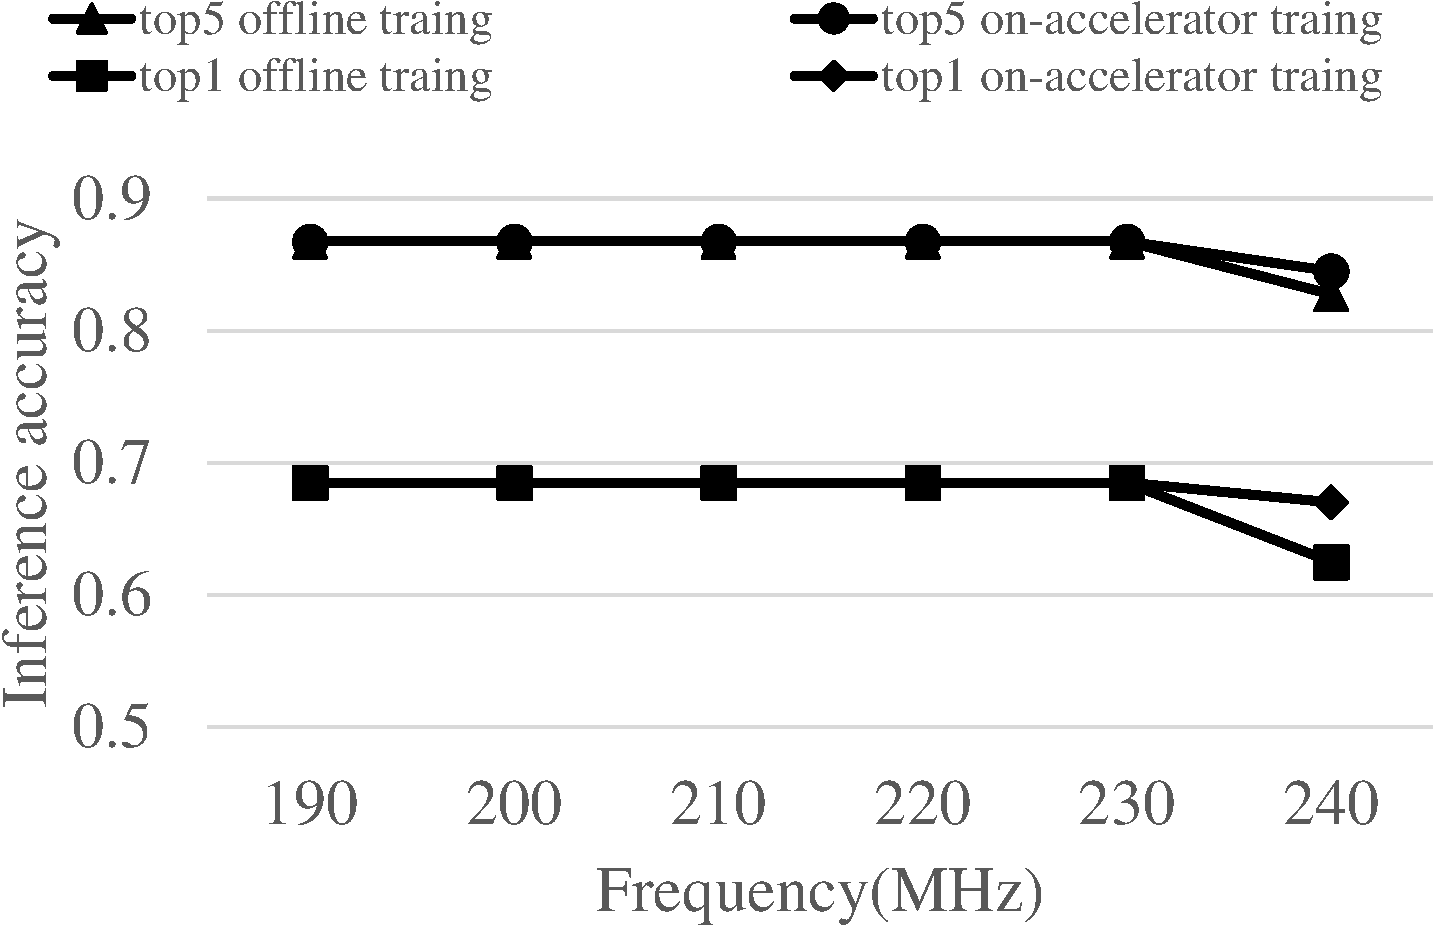
\includegraphics[width=0.6\linewidth]{vgg16_accuracy}
        }
        \qquad
	\subfloat[VGG-19]{
                \label{fig:vgg19_accuracy}
                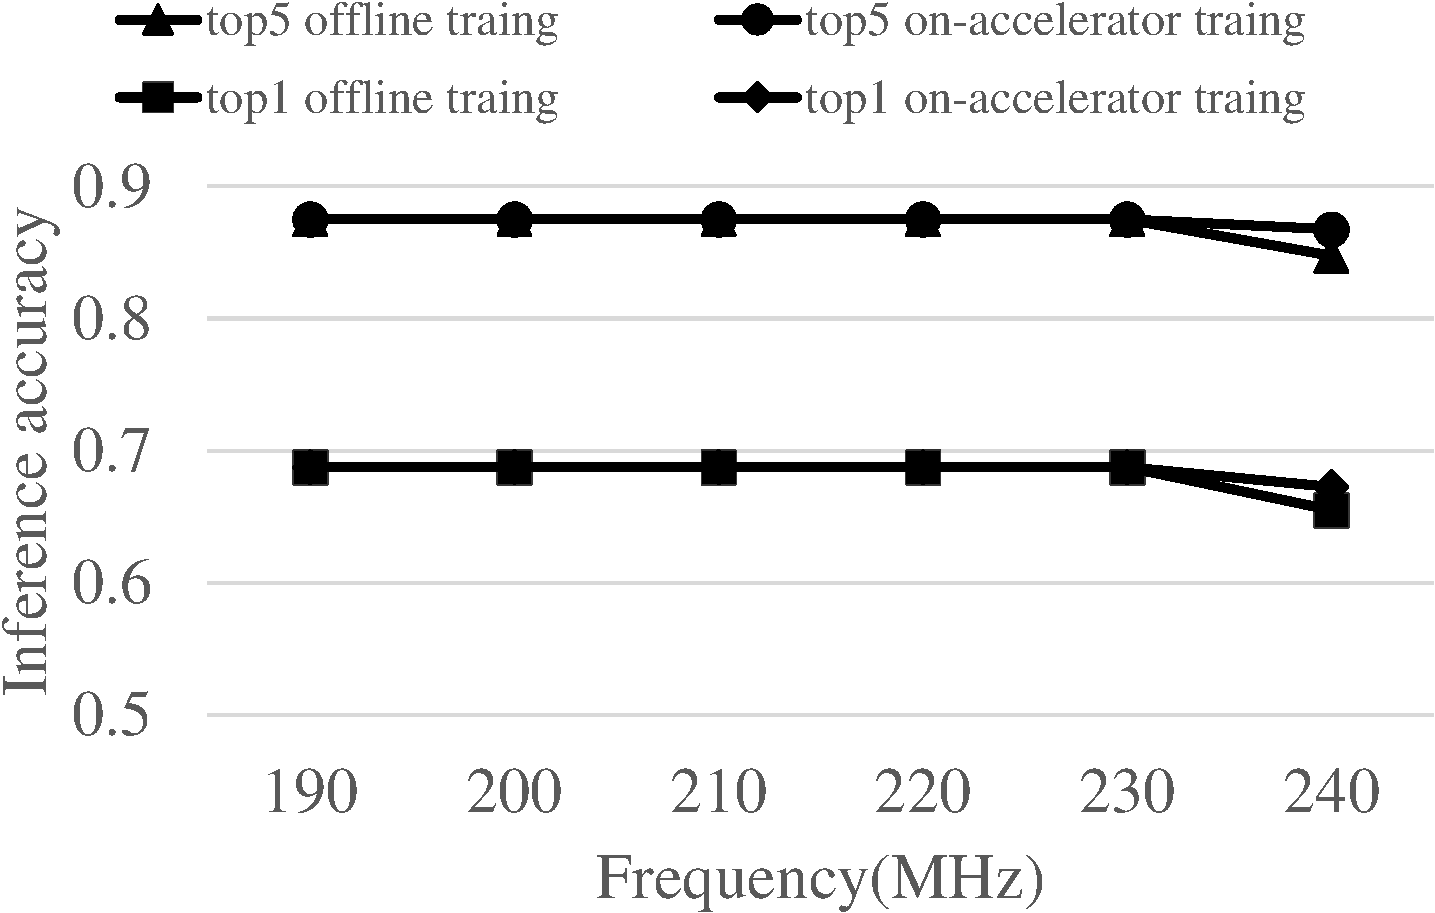
\includegraphics[width=0.6\linewidth]{vgg19_accuracy}
        }
	\caption{The prediction accuracy of the benchmark neural networks on accelerators with different overclocking}
        \label{fig:overclock-accuracy}
\end{figure}

We further evaluate the normalized performance over the original CNN accelerators.
As given in Fig xxx, it can be found that the performance with the extreme accelerator 
overclocking is 1.X on average. With Xilinx power estimator, we also compare the 
power consumption of the CNN accelerators with different overclocking as shown in Fig xxx.
Finally, we use energy-delay product as the energy efficiency metric and compare the 
different overclocking configurations. The comparison is exhibited in Fig xxx.
According to the comparison, we can conclude that overclocking on FPGA based CNN 
accelerators improves both performance and energy efficiency with negligible or small 
predication accuracy loss. In addition, the experiments exhibit that prediction 
accuracy has a cliff-like drop with the increasing overclocking frequency. 

In order to quantize the exact computing errors caused by overclocking, we 
particularly analyze the last layer output of the nerual networks which 
is typically a vector. We compare it with the output without overclocking.
And we use the perceantage of changed output data and the Euclidean distance to 
characterize the difference of the output vector. The comparison is shown in Fig xxx.

\begin{figure}
	\center{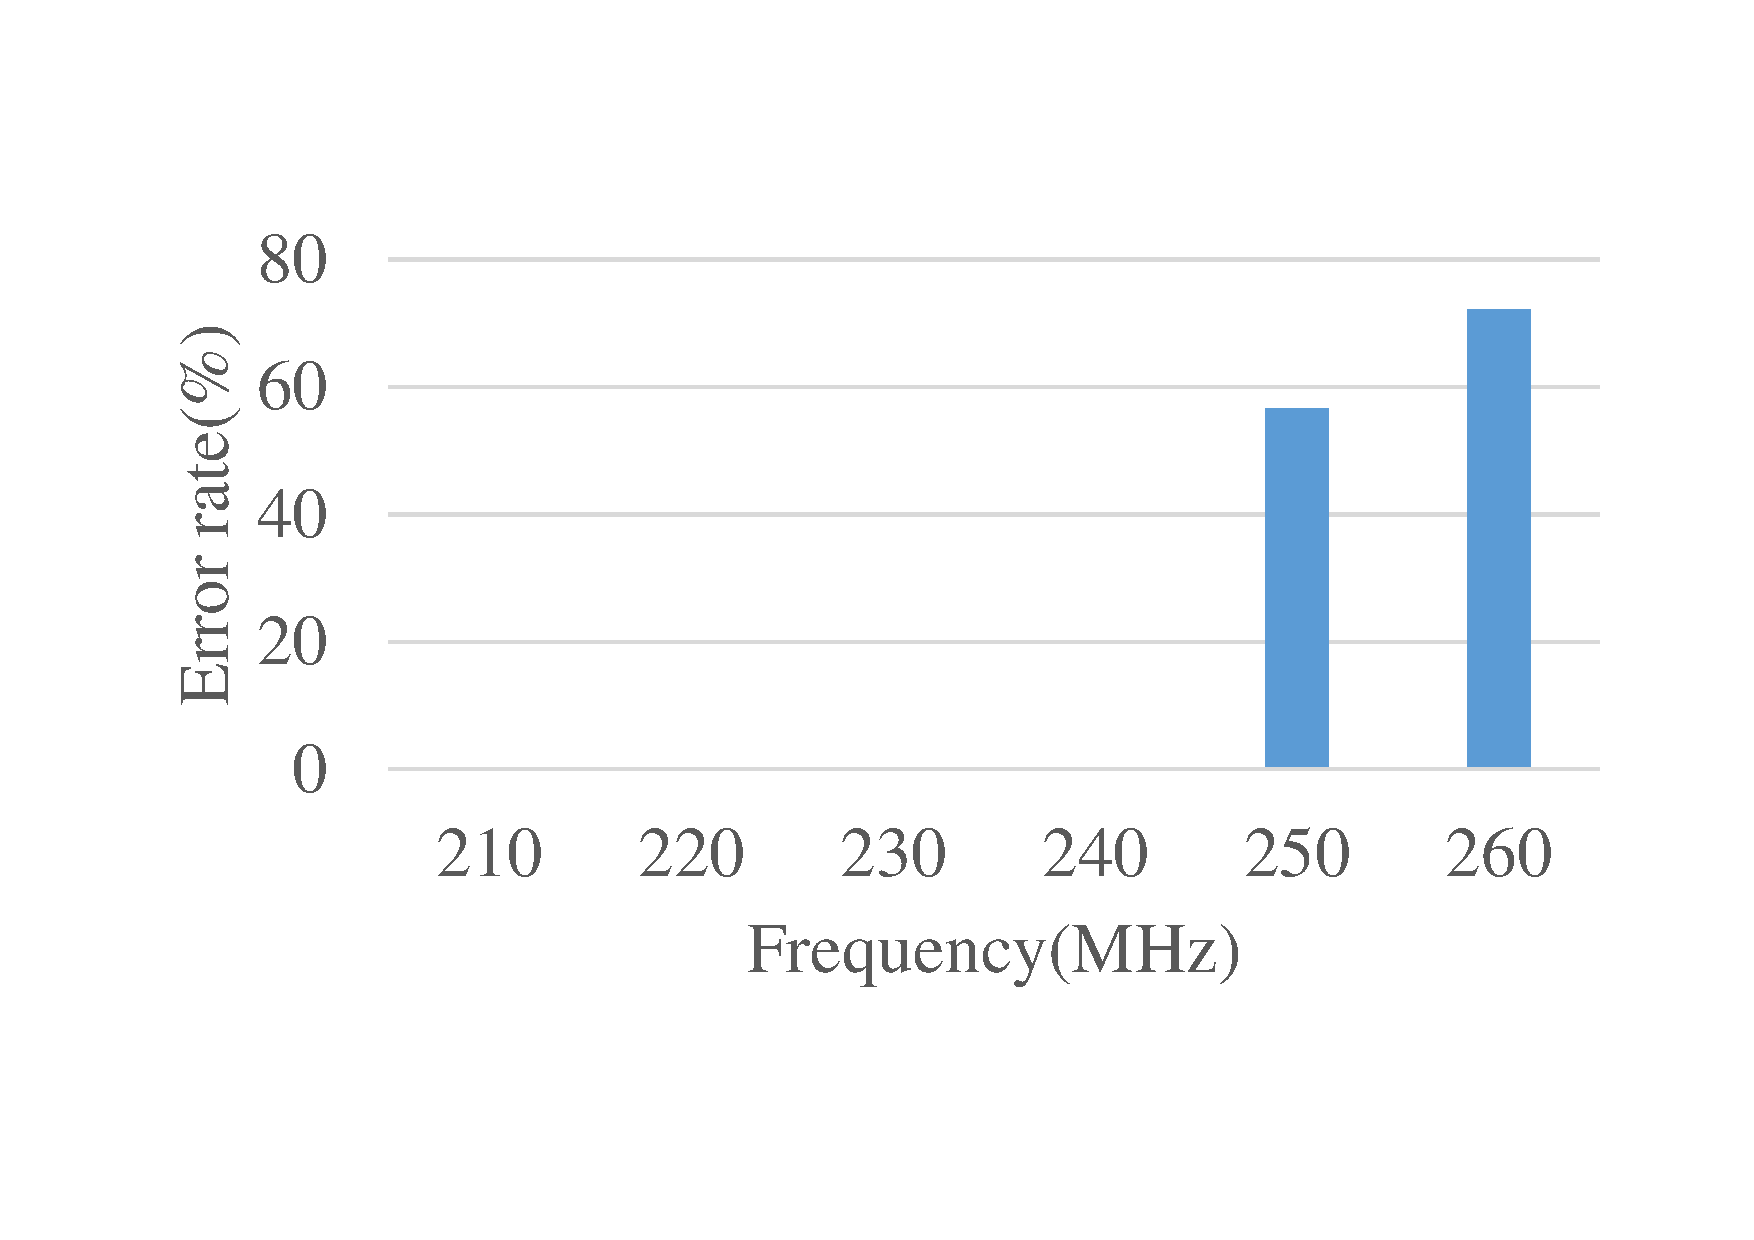
\includegraphics[width=0.75\linewidth]{cuowulv}}
    \caption{Fault rate on the last output layer of the neural network.}
\label{fig:fault_rate}
\vspace{-1em}
\end{figure}

\begin{figure}
	\center{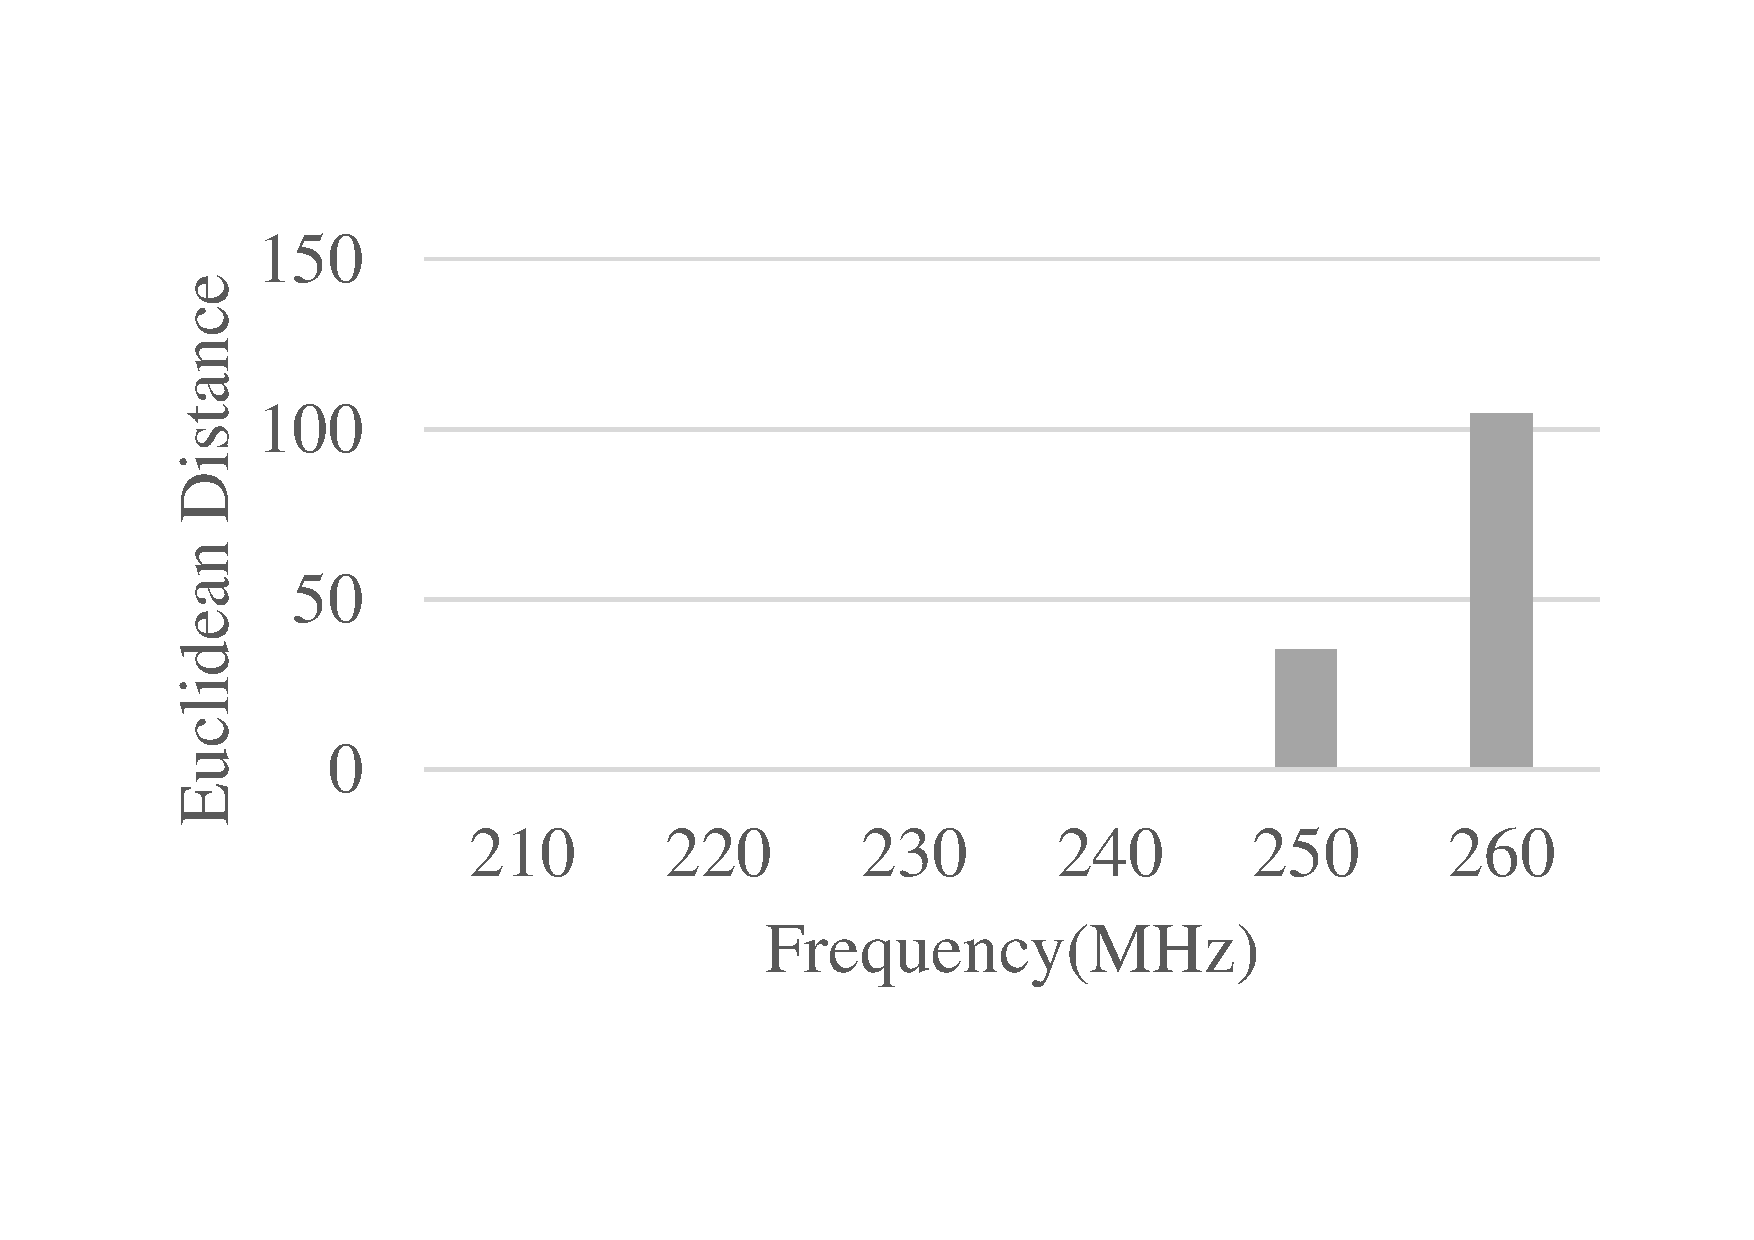
\includegraphics[width=0.75\linewidth]{oushijuli}}
    \caption{Euclidean distance between the acutal output layer and reference output layer.}
\label{fig:euclidean_distance}
\vspace{-1em}
\end{figure}

As discussed in this paper, the timing error can be affected by many factors and it may change 
at runtime. There is no guarantee that the behavior of the CNN accelerator can keep stable even 
overclocking is just slighly higher than the original clock. We use the accelertor overclcoked at the 
tipping point to perform the neural network computing. Then we keep measuring its 
prediction accuracy. As shown in Fig xxx, we find that the accuracy is rather stable.
Although we still can not ensure the stability of the overclocked CNN accelerator, we can 
be sure that the probability of the sever errors such as accelerator hangup or considerable 
accuracy loss is rather low. As we did not observe the cases after processing 1000000 pictuers, 
we assume the probablity of an severe error when processing an input picture is lower than 1/100000.
\begin{figure}
	\center{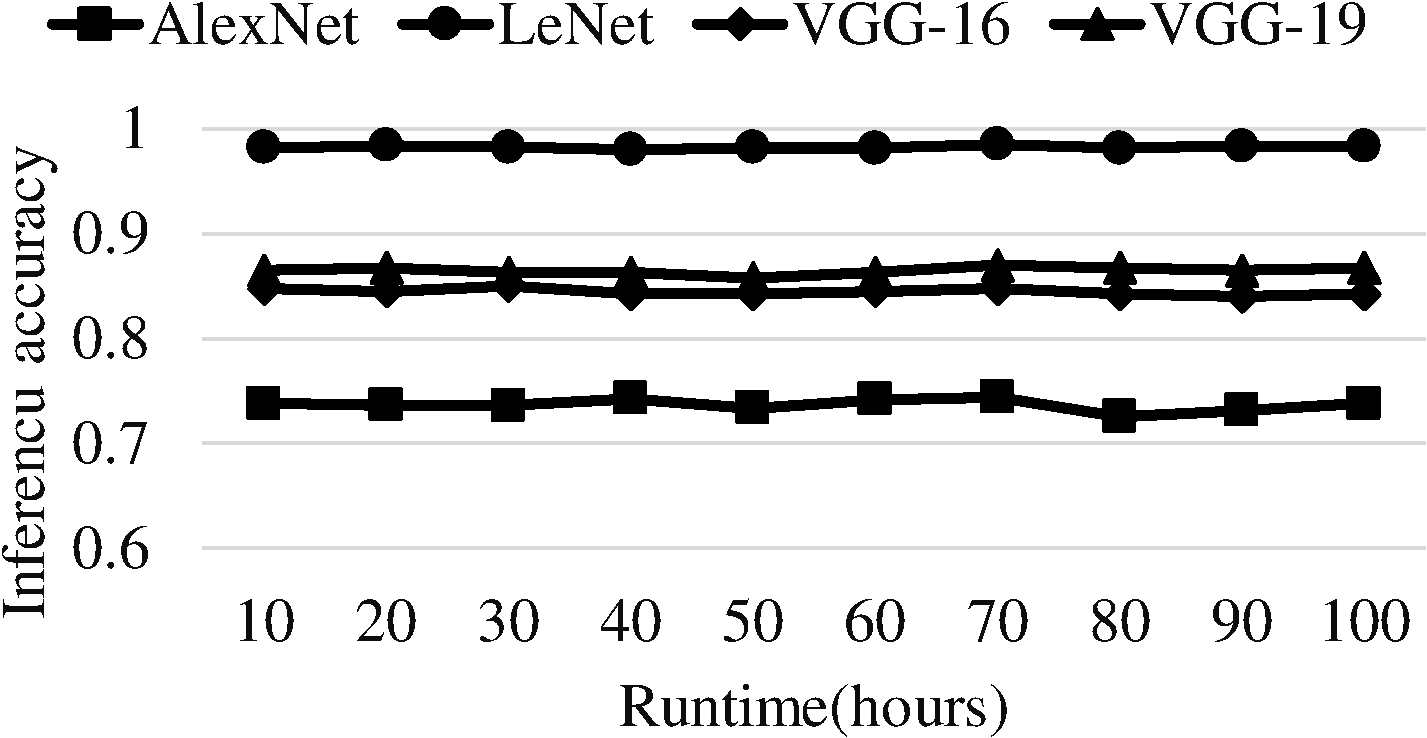
\includegraphics[width=0.75\linewidth]{stability}}
    \caption{Overclocking stability analysis}
\label{fig:stability}
\vspace{-1em}
\end{figure}


\subsection{Optimization tradeoffs}
With the severe error probability, we further evaluate overhead of 
the proposed error detection and error recovery strategy.

